\label{sec:voterflow}

\begin{figure*}
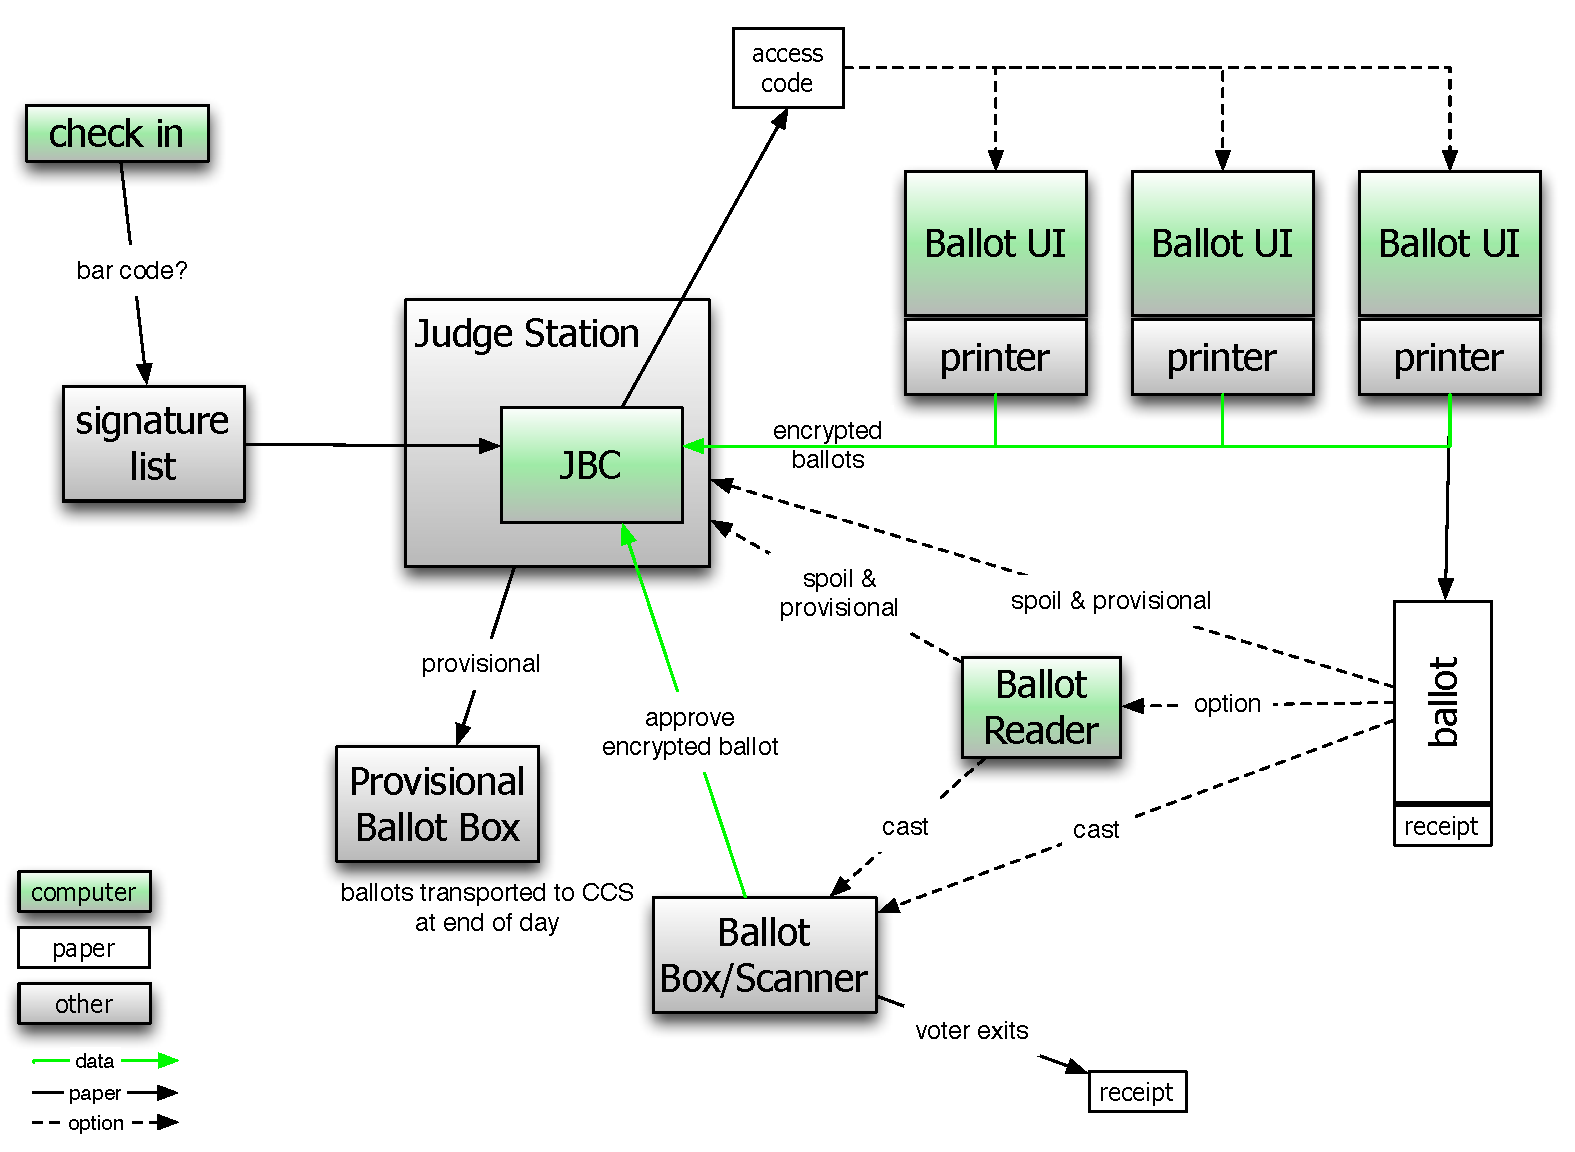
\includegraphics[width=6.5in]{TravisVote.pdf}
\caption{The design of the \projname system. Green objects are computers, white objects are paper records, and other objects are shaded in gray. Arrows display the flow of information; green for digital information, black for paper, and dashed lines indicate that the flow is contingent on voter choice.\label{fig:design}.}
\end{figure*}

Figure~\ref{fig:design} shows how \projname works from the perspective
of a voter going through the system. 
The \projname voting system bears a resemblance to the Hart InterCivic eSlate system and to VoteBox~\cite{sandler08votebox}, in that the voting machines are networked together, 
simplifying the movement of data. 
Like eSlate, our design contains a networked group of voting machines that share a common judge's station with a computer like Hart InterCivic's ``Judge Booth Controller'' (JBC) that manages everything. 

\begin{enumerate}
\item {\em Check-in (pollbook).}
The first step for the voter is to check-in with a poll worker. This is where voter registration is verified and the voter's precinct is identified so that the appropriate ballot style can be generated. The voter also signs into some sort of paper book. Subsequently, the voter will receive something to take to the judge's station that identifies the proper ballot style for the voter. If the voter's registration cannot be verified, a provisional ballot will be used. Notably, {\em there will not be an electronic path between the voter registration phase and subsequent phases}.\footnote{
It would actually be possible to allow provisional voters to vote along with other voters uses the STAR sytem and tag the record for posible later removal, but for simplicity we do not include this process herein.}
Instead, the token, likely from a thermal printer, will only offer a number to identify the ballot style. This might also be encoded as a one-dimensional bar code to reduce data entry errors. Nothing on this token is secret, nor is it unique to any individual voter.

\item {\em Receive token.}
The voter takes the ballot-style identifying token to a poll worker at the judge's station which then issues another token, again probably a piece of paper with a 5-digit code on it. (There will probably need to be a special alternative for ADA compliance as not all voters can see or handle paper.) 

\item {\em Select machine.}
The voter possibly queues at this point, and then selects from one of the available voting stations.

\item  {\em Enter token.}
The first thing the voter does at the voting station is enter the digits on the token. 
This action, in turn indicates the voter's authenticity and identifies the desired ballot style. The token will also be flagged as provisional if that applies. 
Once the voter enters the code, it's transmitted over the local network to the judge's station, invalidating it immediately. Only a small number of these codes will ever be active at any time, allowing codes to be generated randomly and reused through the day. 
There will be no permanent record binding this code to the voter, as that could compromise voter anonymity.\footnote{Hart InterCivic generates comparable codes, but they're not random. Every voter's code is unique to that voter / judge station combination. \projname fixes this problem.}

\item {\em Make selections.}
 The voter makes selections on the GUI (for sighted voters)
 or auditory UI (for non-sighted voters).
 There is a review screen (or the auditory equivalent)
 so that the voter can confirm all selections before producing a paper record.

\item {\em Print.} When the voter has finished making selections,
  the voting terminal prints two (possibly joined) items:
  (1) a paper ballot which includes a human-readable summary of the voter's selections
  and a random (non-sequential) serial number, and
  (2) a paper a take-home receipt that identifies the voting terminal used, the
  time of the vote, and a short (16-20 character) hash code which
  serves as a commitment to the vote but does not reveal its contents.
  The voting terminal also sends data about the vote and receipt
  to the judge's station.\footnote{
  Specifically, the voting terminal sends the judge's station
  the raw ballot selections, an encryption of the ballot selections,
  the hash code derived from this encryption
  which is printed on the voter's take-home receipt,
  and the serial number which is printed on the paper ballot summary.} 


 
  % \COP{Proposal of a variant. There ciphertexts to print are too long
    % when using a homomorphic tallying + we do not want any
    % recognizable link between paper ballots and paper receipts:
% 
% \item {\em Print.} When the voter has finished making selections, she
  % tells the UI to print a paper record of their selections. This
  % cryptographically commits the choices and sends their encrypted
  % ballot to the judge's station as well as printing a paper record, which includes
  % not only a human-readable summary of the voter's selections but a
  % unique serial number (as a bar code or something similar) and a
  % human-readable crypto receipt (essentially a ballot ID number).  }

\item {\em Review printed record.}
The voter may then review the printed record to confirm the indicated selections. There will be at least one station available that can OCR the paper record and read it back to the voter for those who cannot visually read the paper record.

\item {\em Option: Cast or challenge/spoil.}
After reviewing the ballot, the voter has a choice: Cast the ballot or spoil it.
 A voter might spoil the ballot because of an error (or change of heart)
 or because the voter wishes to challenge the voting terminal, demanding it to show
 that the voter's selections were correctly recorded and committed to.\footnote{
 This follows the cryptographic verification process introduced by Benaloh
 in \cite{benaloh06simple} and \cite{benaloh07evt}.}
 The two procedures are described below. Note also that there is a special procedure for provisional ballots.

 Regardless of which case, the voter may keep the take-home paper receipt.
 We note that most thermal printers include a cutting device that leaves a
 small paper connection between the two sides of the cut.
 It is therefore a simple matter for the voting terminal to print a single
 sheet that the voter can easily separate into the ballot summary and the
 take-home receipt.
 We also note that ``privacy sleeves'' (i.e., simple paper folders) can protect the privacy of these printed ballots as voters carry them from the voting machine to either the ballot box, to be cast, or the judge's station, to be spoiled.

\begin{enumerate}
\item  {\em Cast ballot.}
A voter who wishes to cast the ballot takes the paper ballot summary to the ballot box.
% The voter optionally removes the receipt and drops it into the box, where the bar code on the record is scanned.
The ballot box has a simple scanner that can read the serial number from the ballot
(the serial number might also be represented as a one-dimensional barcode for reliability)
and communicate this to the judge's station, allowing the judge's station to keep a record of which ballots have found their way to the ballot box, and thus, which ballots should be tabulated. 
{\em An electronic ballot record is not considered complete and should not be
 included in the tally unless and until its corresponding paper ballot summary has
 been deposited in the balot box.}

\item {\em Spoil ballot.}
If the paper record is to be spoiled, the voter returns to a poll worker at a judge's station. 
% The record will be placed in a special sleeve so that the poll worker cannot see the selections.
The ballot serial number is scanned so that the judge's station can record that the ballot is to be spoiled. Furthermore, the judge's station knows that the corresponding encrypted ballot record should never be used in a real tally. 
Instead, it should be decrypted and published as such. 
The original printed paper ballot thus corresponds to a {\em commitment\/} by the voting machine, before it ever knew it might be challenged.
 If the voting machine cannot produce a suitable proof that the ballot encryption matches the plaintext,
 then it's been caught cheating.
 Of course, for voters who don't care about verification,
 they can simply restart the process.
 For voters who may feel uncomfortable with this process,
 as it might reveal their intent to a poll worker,
 we note that voters could deliberately spoil ballots that misstate their true intent. We note that dedicated election monitors could be allowed to use voting machines, producing printed ballots that they would be forbidden from placing in the ballot box, but which would be spoiled and then the corresponding ciphertext would be decrypted. In effect, election monitors can conduct {\em parallel testing in the field\/} on any voting machine at any time during the live election.


\item {\em Provisional ballot.}
In the case of a provisional ballot, the voter does not have the cast vs.~spoil option, and must return the ballot to a poll worker, who places it into a distinct provisional ballot box. The voter may retain the receipt to see if the ballot ends up being counted.
\end{enumerate}

\item {\em At home (optional): Voter checks crypto.}
The encrypted votes will be posted on a public ``bulletin board''
 (i.e., a web site maintained by the county).
 The voter receipt corresponds to a cryptographic hash of the encrypted vote.
 A voter should be able to easily verify that this vote is present on the bulletin board.
 If a voter spoiled a ballot, that should also be visible on the bulletin board
 together with its decrypted selections.  This allows independent observers to
 know which ballots to include in the tally and allows independent verifiers
 to check that all spoiled ballots are correctly decrypted.  Individual voters can
 check, without any mathematics,
 that the decryptions of their own spoiled ballots match their expectations.
\end{enumerate}

% << sections 2.2 and 3 should go in here somewhere >>


%%% Local Variables: 
%%% mode: latex
%%% TeX-master: "star"
%%% End: 
